\PassOptionsToPackage{unicode=true}{hyperref} % options for packages loaded elsewhere
\PassOptionsToPackage{hyphens}{url}
%
\documentclass[]{article}
\usepackage{lmodern}
\usepackage{amssymb,amsmath}
\usepackage{ifxetex,ifluatex}
\usepackage{fixltx2e} % provides \textsubscript
\ifnum 0\ifxetex 1\fi\ifluatex 1\fi=0 % if pdftex
  \usepackage[T1]{fontenc}
  \usepackage[utf8]{inputenc}
  \usepackage{textcomp} % provides euro and other symbols
\else % if luatex or xelatex
  \usepackage{unicode-math}
  \defaultfontfeatures{Ligatures=TeX,Scale=MatchLowercase}
\fi
% use upquote if available, for straight quotes in verbatim environments
\IfFileExists{upquote.sty}{\usepackage{upquote}}{}
% use microtype if available
\IfFileExists{microtype.sty}{%
\usepackage[]{microtype}
\UseMicrotypeSet[protrusion]{basicmath} % disable protrusion for tt fonts
}{}
\IfFileExists{parskip.sty}{%
\usepackage{parskip}
}{% else
\setlength{\parindent}{0pt}
\setlength{\parskip}{6pt plus 2pt minus 1pt}
}
\usepackage{hyperref}
\hypersetup{
            pdftitle={Testing Report},
            pdfauthor={Group 5: Xujie Ma, Yiqi Lei, Xinyi Zhang, Jiaqi Yuan, Yue Liang},
            pdfborder={0 0 0},
            breaklinks=true}
\urlstyle{same}  % don't use monospace font for urls
\usepackage[margin=1in]{geometry}
\usepackage{color}
\usepackage{fancyvrb}
\newcommand{\VerbBar}{|}
\newcommand{\VERB}{\Verb[commandchars=\\\{\}]}
\DefineVerbatimEnvironment{Highlighting}{Verbatim}{commandchars=\\\{\}}
% Add ',fontsize=\small' for more characters per line
\usepackage{framed}
\definecolor{shadecolor}{RGB}{248,248,248}
\newenvironment{Shaded}{\begin{snugshade}}{\end{snugshade}}
\newcommand{\AlertTok}[1]{\textcolor[rgb]{0.94,0.16,0.16}{#1}}
\newcommand{\AnnotationTok}[1]{\textcolor[rgb]{0.56,0.35,0.01}{\textbf{\textit{#1}}}}
\newcommand{\AttributeTok}[1]{\textcolor[rgb]{0.77,0.63,0.00}{#1}}
\newcommand{\BaseNTok}[1]{\textcolor[rgb]{0.00,0.00,0.81}{#1}}
\newcommand{\BuiltInTok}[1]{#1}
\newcommand{\CharTok}[1]{\textcolor[rgb]{0.31,0.60,0.02}{#1}}
\newcommand{\CommentTok}[1]{\textcolor[rgb]{0.56,0.35,0.01}{\textit{#1}}}
\newcommand{\CommentVarTok}[1]{\textcolor[rgb]{0.56,0.35,0.01}{\textbf{\textit{#1}}}}
\newcommand{\ConstantTok}[1]{\textcolor[rgb]{0.00,0.00,0.00}{#1}}
\newcommand{\ControlFlowTok}[1]{\textcolor[rgb]{0.13,0.29,0.53}{\textbf{#1}}}
\newcommand{\DataTypeTok}[1]{\textcolor[rgb]{0.13,0.29,0.53}{#1}}
\newcommand{\DecValTok}[1]{\textcolor[rgb]{0.00,0.00,0.81}{#1}}
\newcommand{\DocumentationTok}[1]{\textcolor[rgb]{0.56,0.35,0.01}{\textbf{\textit{#1}}}}
\newcommand{\ErrorTok}[1]{\textcolor[rgb]{0.64,0.00,0.00}{\textbf{#1}}}
\newcommand{\ExtensionTok}[1]{#1}
\newcommand{\FloatTok}[1]{\textcolor[rgb]{0.00,0.00,0.81}{#1}}
\newcommand{\FunctionTok}[1]{\textcolor[rgb]{0.00,0.00,0.00}{#1}}
\newcommand{\ImportTok}[1]{#1}
\newcommand{\InformationTok}[1]{\textcolor[rgb]{0.56,0.35,0.01}{\textbf{\textit{#1}}}}
\newcommand{\KeywordTok}[1]{\textcolor[rgb]{0.13,0.29,0.53}{\textbf{#1}}}
\newcommand{\NormalTok}[1]{#1}
\newcommand{\OperatorTok}[1]{\textcolor[rgb]{0.81,0.36,0.00}{\textbf{#1}}}
\newcommand{\OtherTok}[1]{\textcolor[rgb]{0.56,0.35,0.01}{#1}}
\newcommand{\PreprocessorTok}[1]{\textcolor[rgb]{0.56,0.35,0.01}{\textit{#1}}}
\newcommand{\RegionMarkerTok}[1]{#1}
\newcommand{\SpecialCharTok}[1]{\textcolor[rgb]{0.00,0.00,0.00}{#1}}
\newcommand{\SpecialStringTok}[1]{\textcolor[rgb]{0.31,0.60,0.02}{#1}}
\newcommand{\StringTok}[1]{\textcolor[rgb]{0.31,0.60,0.02}{#1}}
\newcommand{\VariableTok}[1]{\textcolor[rgb]{0.00,0.00,0.00}{#1}}
\newcommand{\VerbatimStringTok}[1]{\textcolor[rgb]{0.31,0.60,0.02}{#1}}
\newcommand{\WarningTok}[1]{\textcolor[rgb]{0.56,0.35,0.01}{\textbf{\textit{#1}}}}
\usepackage{longtable,booktabs}
% Fix footnotes in tables (requires footnote package)
\IfFileExists{footnote.sty}{\usepackage{footnote}\makesavenoteenv{longtable}}{}
\usepackage{graphicx,grffile}
\makeatletter
\def\maxwidth{\ifdim\Gin@nat@width>\linewidth\linewidth\else\Gin@nat@width\fi}
\def\maxheight{\ifdim\Gin@nat@height>\textheight\textheight\else\Gin@nat@height\fi}
\makeatother
% Scale images if necessary, so that they will not overflow the page
% margins by default, and it is still possible to overwrite the defaults
% using explicit options in \includegraphics[width, height, ...]{}
\setkeys{Gin}{width=\maxwidth,height=\maxheight,keepaspectratio}
\setlength{\emergencystretch}{3em}  % prevent overfull lines
\providecommand{\tightlist}{%
  \setlength{\itemsep}{0pt}\setlength{\parskip}{0pt}}
\setcounter{secnumdepth}{0}
% Redefines (sub)paragraphs to behave more like sections
\ifx\paragraph\undefined\else
\let\oldparagraph\paragraph
\renewcommand{\paragraph}[1]{\oldparagraph{#1}\mbox{}}
\fi
\ifx\subparagraph\undefined\else
\let\oldsubparagraph\subparagraph
\renewcommand{\subparagraph}[1]{\oldsubparagraph{#1}\mbox{}}
\fi

% set default figure placement to htbp
\makeatletter
\def\fps@figure{htbp}
\makeatother


\title{Testing Report}
\author{Group 5: Xujie Ma, Yiqi Lei, Xinyi Zhang, Jiaqi Yuan, Yue Liang}
\date{11/26/2020}

\begin{document}
\maketitle

In this notebook, we are presenting 3 algorithms:

\begin{enumerate}
\def\labelenumi{\arabic{enumi}.}
\item
  14 A3+P5 Doubly Robust Estimation + boosted stumps
\item
  21 A6+P5 Regression Adjustment + boosted stumps
\item
  15 A4 Regression Estimate
\end{enumerate}

\hypertarget{data-import}{%
\subsection{Data Import}\label{data-import}}

\begin{Shaded}
\begin{Highlighting}[]
\NormalTok{high <-}\StringTok{ }\KeywordTok{read.csv}\NormalTok{(}\StringTok{'../data/highDim_dataset.csv'}\NormalTok{)}
\NormalTok{low <-}\StringTok{ }\KeywordTok{read.csv}\NormalTok{(}\StringTok{'../data/lowDim_dataset.csv'}\NormalTok{)}
\end{Highlighting}
\end{Shaded}

\hypertarget{algo-1-14-a3p5-doubly-robust-estimation-boosted-stumps}{%
\section{Algo 1: 14 A3+P5 Doubly Robust Estimation + boosted
stumps}\label{algo-1-14-a3p5-doubly-robust-estimation-boosted-stumps}}

\hypertarget{methodology-and-implementation}{%
\subsection{Methodology and
Implementation}\label{methodology-and-implementation}}

\begin{enumerate}
\def\labelenumi{\arabic{enumi}.}
\tightlist
\item
  Reference: {[}1{]} Chan D , Ge R , Gershony O , et al.~Evaluating
  online ad campaigns in a pipeline: causal models at scale{[}C{]}// Acm
  Sigkdd International Conference on Knowledge Discovery \& Data Mining.
  ACM, 2010. {[}2{]} Lunceford, Jared K . Stratification and weighting
  via the propensity score in estimation of causal treatment effects: a
  comparative study{[}J{]}. Statistics in Medicine, 2017.
\item
  Doubly Robust Estimation
\end{enumerate}

\begin{itemize}
\tightlist
\item
  What is it: It is a method to estimate treatment effect. Doubly robust
  estimator has the smallest asymptotic variance. ``Doubly robust'' in
  the sense that the estimator remains consistent if either (i) if the
  propensity score model is correctly specified but the two regression
  models m0 and m1 are not or (ii) the two regression models are
  correctly specified but the propensity score model is not, although
  under these conditions it might not be the most efficient.
\item
  Implementation: ATE=E{[}E(Y\textbar{}T =1,X)−E(Y\textbar{}T
  =0,X){]}+E{[}I(T=1)/propensity\_score-I(T=0)/(1-propensity\_score)(Y-E(Y\textbar{}T,X)){]},
  in which E(Y \textbar{}T = t, X) is usually obtained by regressing the
  observed response Y on X in group t (where t = 0,1).
\end{itemize}

\hypertarget{highdim_dataset}{%
\subsection{HighDim\_dataset}\label{highdim_dataset}}

\begin{Shaded}
\begin{Highlighting}[]
\CommentTok{# train-test split}
\NormalTok{n <-}\StringTok{ }\KeywordTok{nrow}\NormalTok{(high)}
\NormalTok{n_train <-}\StringTok{ }\KeywordTok{round}\NormalTok{(n}\OperatorTok{*}\NormalTok{(}\DecValTok{4}\OperatorTok{/}\DecValTok{5}\NormalTok{),}\DecValTok{0}\NormalTok{)}
\NormalTok{train_idx <-}\StringTok{ }\KeywordTok{sample}\NormalTok{(}\DecValTok{1}\OperatorTok{:}\NormalTok{n,n_train)}
\NormalTok{train_high <-}\StringTok{ }\NormalTok{high[train_idx,]}
\NormalTok{test_high <-}\StringTok{ }\NormalTok{high[}\OperatorTok{-}\NormalTok{train_idx,]}

\CommentTok{#Split treatment and control group, and complete regression for each group.}
\NormalTok{treatment.group.high<-high[high}\OperatorTok{$}\NormalTok{A}\OperatorTok{==}\DecValTok{1}\NormalTok{,}\OperatorTok{-}\DecValTok{2}\NormalTok{]}
\NormalTok{control.group.high<-high[high}\OperatorTok{$}\NormalTok{A}\OperatorTok{==}\DecValTok{0}\NormalTok{,}\OperatorTok{-}\DecValTok{2}\NormalTok{]}

\NormalTok{treatment.model.high<-}\KeywordTok{lm}\NormalTok{(Y}\OperatorTok{~}\NormalTok{.,}\DataTypeTok{data=}\NormalTok{treatment.group.high)}
\NormalTok{control.model.high<-}\KeywordTok{lm}\NormalTok{(Y}\OperatorTok{~}\NormalTok{.,}\DataTypeTok{data=}\NormalTok{control.group.high)}

\CommentTok{# Estimate m1(X) and m0(X) for all entries.}
\NormalTok{X.high<-high[}\OperatorTok{-}\KeywordTok{c}\NormalTok{(}\DecValTok{1}\NormalTok{,}\DecValTok{2}\NormalTok{)]}

\NormalTok{high}\OperatorTok{$}\NormalTok{m1<-}\KeywordTok{predict}\NormalTok{(treatment.model.high,X.high)}
\NormalTok{high}\OperatorTok{$}\NormalTok{m0<-}\KeywordTok{predict}\NormalTok{(control.model.high,X.high)}
\end{Highlighting}
\end{Shaded}

Get propensity score for all entries using boosted stumps (Gradient
Boosting Machine).

Using grid search to get proper parameters for gbm.

\begin{Shaded}
\begin{Highlighting}[]
\CommentTok{# grid search}
\NormalTok{hyper_grid_high1 <-}\StringTok{ }\KeywordTok{expand.grid}\NormalTok{(}
  \DataTypeTok{n.trees =} \KeywordTok{c}\NormalTok{(}\DecValTok{40}\NormalTok{,}\DecValTok{50}\NormalTok{,}\DecValTok{60}\NormalTok{),}
  \DataTypeTok{shrinkage =} \KeywordTok{c}\NormalTok{(.}\DecValTok{01}\NormalTok{, }\FloatTok{.05}\NormalTok{, }\FloatTok{.1}\NormalTok{),}
  \DataTypeTok{n.minobsinnode =} \KeywordTok{c}\NormalTok{(}\DecValTok{5}\NormalTok{, }\DecValTok{10}\NormalTok{, }\DecValTok{15}\NormalTok{),}
  \DataTypeTok{bag.fraction =} \KeywordTok{c}\NormalTok{(.}\DecValTok{65}\NormalTok{, }\FloatTok{.8}\NormalTok{, }\DecValTok{1}\NormalTok{), }
  \DataTypeTok{optimal_trees =} \DecValTok{0}\NormalTok{,               }\CommentTok{# a place to dump results}
  \DataTypeTok{min_RMSE =} \DecValTok{0}                     \CommentTok{# a place to dump results}
\NormalTok{)}

\CommentTok{# randomize data}
\NormalTok{random_index <-}\StringTok{ }\KeywordTok{sample}\NormalTok{(}\DecValTok{1}\OperatorTok{:}\KeywordTok{nrow}\NormalTok{(train_high), }\KeywordTok{nrow}\NormalTok{(train_high))}
\NormalTok{random_ames_train <-}\StringTok{ }\NormalTok{train_high[random_index, ]}

\CommentTok{# grid search }
\ControlFlowTok{for}\NormalTok{(i }\ControlFlowTok{in} \DecValTok{1}\OperatorTok{:}\KeywordTok{nrow}\NormalTok{(hyper_grid_high1)) \{}
  \CommentTok{# reproducibility}
  \KeywordTok{set.seed}\NormalTok{(}\DecValTok{2020}\NormalTok{)}
  \CommentTok{# train model}
\NormalTok{  gbm.tune <-}\StringTok{ }\KeywordTok{gbm}\NormalTok{(}
    \DataTypeTok{formula =}\NormalTok{ A}\OperatorTok{~}\NormalTok{.,}
    \DataTypeTok{distribution =} \StringTok{"bernoulli"}\NormalTok{,}
    \DataTypeTok{data =}\NormalTok{ train_high[}\OperatorTok{-}\DecValTok{1}\NormalTok{],}
    \DataTypeTok{n.trees =}\NormalTok{ hyper_grid_high1}\OperatorTok{$}\NormalTok{n.trees[i],}
    \DataTypeTok{interaction.depth =} \DecValTok{1}\NormalTok{,}
    \DataTypeTok{shrinkage =}\NormalTok{ hyper_grid_high1}\OperatorTok{$}\NormalTok{shrinkage[i],}
    \DataTypeTok{n.minobsinnode =}\NormalTok{ hyper_grid_high1}\OperatorTok{$}\NormalTok{n.minobsinnode[i],}
    \DataTypeTok{bag.fraction =}\NormalTok{ hyper_grid_high1}\OperatorTok{$}\NormalTok{bag.fraction[i],}
    \DataTypeTok{train.fraction =} \FloatTok{.75}
\NormalTok{  )}
  
  \CommentTok{# add min training error and trees to grid}
\NormalTok{  hyper_grid_high1}\OperatorTok{$}\NormalTok{optimal_trees[i] <-}\StringTok{ }\KeywordTok{which.min}\NormalTok{(gbm.tune}\OperatorTok{$}\NormalTok{valid.error)}
\NormalTok{  hyper_grid_high1}\OperatorTok{$}\NormalTok{min_RMSE[i] <-}\StringTok{ }\KeywordTok{sqrt}\NormalTok{(}\KeywordTok{min}\NormalTok{(gbm.tune}\OperatorTok{$}\NormalTok{valid.error))}
\NormalTok{\}}

\NormalTok{hyper_grid_high1 }\OperatorTok\StringTok{ }
\StringTok{  }\NormalTok{dplyr}\OperatorTok{::}\KeywordTok{arrange}\NormalTok{(min_RMSE) }\OperatorTok
\StringTok{  }\KeywordTok{head}\NormalTok{(}\DecValTok{10}\NormalTok{)}
\end{Highlighting}
\end{Shaded}

Apply the parameters with min\_RMSE (n.trees=60, shrinkage=0.1,
n.minobsinnode=10, bag.fraction=1).

\begin{Shaded}
\begin{Highlighting}[]
\KeywordTok{set.seed}\NormalTok{(}\DecValTok{2020}\NormalTok{) }

\NormalTok{tm_highe1 <-}\StringTok{ }\KeywordTok{system.time}\NormalTok{(}
\NormalTok{  boost.high<-}\KeywordTok{gbm}\NormalTok{(A}\OperatorTok{~}\NormalTok{., }\DataTypeTok{data =}\NormalTok{ train_high[}\OperatorTok{-}\DecValTok{1}\NormalTok{], }
                  \DataTypeTok{distribution =} \StringTok{"bernoulli"}\NormalTok{,}
                   \DataTypeTok{n.trees =} \DecValTok{60}\NormalTok{, }\CommentTok{# the number of trees}
                   \DataTypeTok{shrinkage =} \FloatTok{0.1}\NormalTok{, }\CommentTok{# learning rate}
                   \DataTypeTok{interaction.depth =} \DecValTok{1}\NormalTok{, }\CommentTok{# total split}
                  \DataTypeTok{n.minobsinnode =} \DecValTok{10}\NormalTok{,}
                  \DataTypeTok{bag.fraction =} \DecValTok{1}
\NormalTok{                   )}
\NormalTok{  )}

\CommentTok{# Calculate propensity scores for all entries in high.csv}
\NormalTok{tm_highe2 <-}\StringTok{ }\KeywordTok{system.time}\NormalTok{(}
\NormalTok{  high}\OperatorTok{$}\NormalTok{e <-}\StringTok{ }\KeywordTok{predict}\NormalTok{(boost.high, X.high, }\DataTypeTok{n.trees =} \DecValTok{60}\NormalTok{, }\DataTypeTok{type =} \StringTok{'response'}\NormalTok{)}
\NormalTok{)}

\CommentTok{# Calculate each part in doubly robust estimation and count out the final result.}
\NormalTok{tm_highATE1 <-}\StringTok{ }\KeywordTok{system.time}\NormalTok{(}
\NormalTok{  \{high}\OperatorTok{$}\NormalTok{p1<-}\KeywordTok{ifelse}\NormalTok{(high}\OperatorTok{$}\NormalTok{A}\OperatorTok{==}\DecValTok{1}\NormalTok{,(high}\OperatorTok{$}\NormalTok{Y}\OperatorTok{-}\NormalTok{high}\OperatorTok{$}\NormalTok{m1)}\OperatorTok{/}\NormalTok{high}\OperatorTok{$}\NormalTok{e,}\DecValTok{0}\NormalTok{);}
\NormalTok{  high}\OperatorTok{$}\NormalTok{p2<-}\KeywordTok{ifelse}\NormalTok{(high}\OperatorTok{$}\NormalTok{A}\OperatorTok{==}\DecValTok{0}\NormalTok{,(high}\OperatorTok{$}\NormalTok{Y}\OperatorTok{-}\NormalTok{high}\OperatorTok{$}\NormalTok{m0)}\OperatorTok{/}\NormalTok{(}\DecValTok{1}\OperatorTok{-}\NormalTok{high}\OperatorTok{$}\NormalTok{e),}\DecValTok{0}\NormalTok{);}
\NormalTok{  high}\OperatorTok{$}\NormalTok{result<-high}\OperatorTok{$}\NormalTok{m1}\OperatorTok{-}\NormalTok{high}\OperatorTok{$}\NormalTok{m0}\OperatorTok{+}\NormalTok{high}\OperatorTok{$}\NormalTok{p1}\OperatorTok{-}\NormalTok{high}\OperatorTok{$}\NormalTok{p2;}
\NormalTok{  ATE.high<-}\KeywordTok{mean}\NormalTok{(high}\OperatorTok{$}\NormalTok{result)\}}
\NormalTok{  )}

\NormalTok{ATE.high}
\end{Highlighting}
\end{Shaded}

\begin{verbatim}
## [1] -2.95861
\end{verbatim}

\begin{Shaded}
\begin{Highlighting}[]
\CommentTok{#alternative function, same result}

\CommentTok{#tm_highATE2 <- system.time(}
\CommentTok{#  ATE.high<-1/n*(sum((high$A*high$Y-(high$A-high$e)*high$m1)/high$e)}
\CommentTok{#            -sum(((1-high$A)*high$Y+(high$A-high$e)*high$m0)/(1-high$e))))}
\CommentTok{#ATE.high}
\end{Highlighting}
\end{Shaded}

\begin{Shaded}
\begin{Highlighting}[]
\CommentTok{# True ATE:}
\NormalTok{true_ATE_high <-}\StringTok{ }\DecValTok{-3}

\CommentTok{# Comparison:}
\NormalTok{true_ATE_high }\OperatorTok{-}\StringTok{ }\NormalTok{ATE.high}
\end{Highlighting}
\end{Shaded}

\begin{verbatim}
## [1] -0.04138961
\end{verbatim}

\begin{Shaded}
\begin{Highlighting}[]
\NormalTok{time_high<-tm_highe1[}\DecValTok{1}\NormalTok{]}\OperatorTok{+}\NormalTok{tm_highe2[}\DecValTok{1}\NormalTok{]}\OperatorTok{+}\NormalTok{tm_highATE1[}\DecValTok{1}\NormalTok{]}
\KeywordTok{cat}\NormalTok{(}\StringTok{"Time for training gbm="}\NormalTok{, tm_highe1[}\DecValTok{1}\NormalTok{], }\StringTok{"s }\CharTok{\textbackslash{}n}\StringTok{"}\NormalTok{)}
\end{Highlighting}
\end{Shaded}

\begin{verbatim}
## Time for training gbm= 0.292 s
\end{verbatim}

\begin{Shaded}
\begin{Highlighting}[]
\KeywordTok{cat}\NormalTok{(}\StringTok{"Time for getting propensity score="}\NormalTok{, tm_highe2[}\DecValTok{1}\NormalTok{], }\StringTok{"s }\CharTok{\textbackslash{}n}\StringTok{"}\NormalTok{)}
\end{Highlighting}
\end{Shaded}

\begin{verbatim}
## Time for getting propensity score= 0.014 s
\end{verbatim}

\begin{Shaded}
\begin{Highlighting}[]
\KeywordTok{cat}\NormalTok{(}\StringTok{"Time for calculating ATE="}\NormalTok{, tm_highATE1[}\DecValTok{1}\NormalTok{], }\StringTok{"s }\CharTok{\textbackslash{}n}\StringTok{"}\NormalTok{)}
\end{Highlighting}
\end{Shaded}

\begin{verbatim}
## Time for calculating ATE= 0 s
\end{verbatim}

\hypertarget{lowdim_dataset}{%
\subsection{LowDim\_dataset}\label{lowdim_dataset}}

\begin{Shaded}
\begin{Highlighting}[]
\CommentTok{# train-test split}
\NormalTok{n <-}\StringTok{ }\KeywordTok{nrow}\NormalTok{(low)}
\NormalTok{n_train <-}\StringTok{ }\KeywordTok{round}\NormalTok{(n}\OperatorTok{*}\NormalTok{(}\DecValTok{4}\OperatorTok{/}\DecValTok{5}\NormalTok{),}\DecValTok{0}\NormalTok{)}
\NormalTok{train_idx <-}\StringTok{ }\KeywordTok{sample}\NormalTok{(}\DecValTok{1}\OperatorTok{:}\NormalTok{n,n_train)}
\NormalTok{train_low <-}\StringTok{ }\NormalTok{low[train_idx,]}
\NormalTok{test_low <-}\StringTok{ }\NormalTok{low[}\OperatorTok{-}\NormalTok{train_idx,]}

\CommentTok{# Split treatment and control group, and complete regression for each group.}
\NormalTok{treatment.group.low<-low[low}\OperatorTok{$}\NormalTok{A}\OperatorTok{==}\DecValTok{1}\NormalTok{,}\OperatorTok{-}\DecValTok{2}\NormalTok{]}
\NormalTok{control.group.low<-low[low}\OperatorTok{$}\NormalTok{A}\OperatorTok{==}\DecValTok{0}\NormalTok{,}\OperatorTok{-}\DecValTok{2}\NormalTok{]}

\NormalTok{treatment.model.low<-}\KeywordTok{lm}\NormalTok{(Y}\OperatorTok{~}\NormalTok{.,}\DataTypeTok{data=}\NormalTok{treatment.group.low)}
\NormalTok{control.model.low<-}\KeywordTok{lm}\NormalTok{(Y}\OperatorTok{~}\NormalTok{.,}\DataTypeTok{data=}\NormalTok{control.group.low)}

\CommentTok{# Estimate m1(X) and m0(X) for all entries.}
\NormalTok{X.low<-low[}\OperatorTok{-}\KeywordTok{c}\NormalTok{(}\DecValTok{1}\NormalTok{,}\DecValTok{2}\NormalTok{)]}

\NormalTok{low}\OperatorTok{$}\NormalTok{m1<-}\KeywordTok{predict}\NormalTok{(treatment.model.low,X.low)}
\NormalTok{low}\OperatorTok{$}\NormalTok{m0<-}\KeywordTok{predict}\NormalTok{(control.model.low,X.low)}
\end{Highlighting}
\end{Shaded}

Get propensity score for all entries using boosted stumps (Gradient
Boosting Machine). Using grid search to get proper parameters for gbm.

\begin{Shaded}
\begin{Highlighting}[]
\CommentTok{# grid search}
\NormalTok{hyper_grid_low1 <-}\StringTok{ }\KeywordTok{expand.grid}\NormalTok{(}
  \DataTypeTok{n.trees =} \KeywordTok{c}\NormalTok{(}\DecValTok{40}\NormalTok{,}\DecValTok{50}\NormalTok{,}\DecValTok{60}\NormalTok{),}
  \DataTypeTok{shrinkage =} \KeywordTok{c}\NormalTok{(.}\DecValTok{01}\NormalTok{, }\FloatTok{.05}\NormalTok{, }\FloatTok{.1}\NormalTok{),}
  \DataTypeTok{n.minobsinnode =} \KeywordTok{c}\NormalTok{(}\DecValTok{5}\NormalTok{, }\DecValTok{10}\NormalTok{, }\DecValTok{15}\NormalTok{),}
  \DataTypeTok{bag.fraction =} \KeywordTok{c}\NormalTok{(.}\DecValTok{65}\NormalTok{, }\FloatTok{.8}\NormalTok{, }\DecValTok{1}\NormalTok{), }
  \DataTypeTok{optimal_trees =} \DecValTok{0}\NormalTok{,               }\CommentTok{# a place to dump results}
  \DataTypeTok{min_RMSE =} \DecValTok{0}                     \CommentTok{# a place to dump results}
\NormalTok{)}

\CommentTok{# randomize data}
\NormalTok{random_index <-}\StringTok{ }\KeywordTok{sample}\NormalTok{(}\DecValTok{1}\OperatorTok{:}\KeywordTok{nrow}\NormalTok{(train_low), }\KeywordTok{nrow}\NormalTok{(train_low))}
\NormalTok{random_ames_train <-}\StringTok{ }\NormalTok{train_low[random_index, ]}

\CommentTok{# grid search }
\ControlFlowTok{for}\NormalTok{(i }\ControlFlowTok{in} \DecValTok{1}\OperatorTok{:}\KeywordTok{nrow}\NormalTok{(hyper_grid_low1)) \{}
  \CommentTok{# reproducibility}
  \KeywordTok{set.seed}\NormalTok{(}\DecValTok{2020}\NormalTok{)}
  \CommentTok{# train model}
\NormalTok{  gbm.tune <-}\StringTok{ }\KeywordTok{gbm}\NormalTok{(}
    \DataTypeTok{formula =}\NormalTok{ A}\OperatorTok{~}\NormalTok{.,}
    \DataTypeTok{distribution =} \StringTok{"bernoulli"}\NormalTok{,}
    \DataTypeTok{data =}\NormalTok{ train_low[}\OperatorTok{-}\DecValTok{1}\NormalTok{],}
    \DataTypeTok{n.trees =}\NormalTok{ hyper_grid_low1}\OperatorTok{$}\NormalTok{n.trees[i],}
    \DataTypeTok{interaction.depth =} \DecValTok{1}\NormalTok{,}
    \DataTypeTok{shrinkage =}\NormalTok{ hyper_grid_low1}\OperatorTok{$}\NormalTok{shrinkage[i],}
    \DataTypeTok{n.minobsinnode =}\NormalTok{ hyper_grid_low1}\OperatorTok{$}\NormalTok{n.minobsinnode[i],}
    \DataTypeTok{bag.fraction =}\NormalTok{ hyper_grid_low1}\OperatorTok{$}\NormalTok{bag.fraction[i],}
    \DataTypeTok{train.fraction =} \FloatTok{0.75}
\NormalTok{  )}
  
  \CommentTok{# add min training error and trees to grid}
\NormalTok{  hyper_grid_low1}\OperatorTok{$}\NormalTok{optimal_trees[i] <-}\StringTok{ }\KeywordTok{which.min}\NormalTok{(gbm.tune}\OperatorTok{$}\NormalTok{valid.error)}
\NormalTok{  hyper_grid_low1}\OperatorTok{$}\NormalTok{min_RMSE[i] <-}\StringTok{ }\KeywordTok{sqrt}\NormalTok{(}\KeywordTok{min}\NormalTok{(gbm.tune}\OperatorTok{$}\NormalTok{valid.error))}
\NormalTok{\}}

\NormalTok{hyper_grid_low1 }\OperatorTok\StringTok{ }
\StringTok{  }\NormalTok{dplyr}\OperatorTok{::}\KeywordTok{arrange}\NormalTok{(min_RMSE) }\OperatorTok
\StringTok{  }\KeywordTok{head}\NormalTok{(}\DecValTok{10}\NormalTok{)}
\end{Highlighting}
\end{Shaded}

Apply the parameters with min\_RMSE (n.trees=60, shrinkage=0.1,
n.minobsinnode=15, bag.fraction=0.8).

\begin{Shaded}
\begin{Highlighting}[]
\KeywordTok{set.seed}\NormalTok{(}\DecValTok{2020}\NormalTok{)}

\NormalTok{tm_lowe1 <-}\StringTok{ }\KeywordTok{system.time}\NormalTok{(}
\NormalTok{boost.low <-}\StringTok{ }\KeywordTok{gbm}\NormalTok{(A}\OperatorTok{~}\NormalTok{., }\DataTypeTok{data =}\NormalTok{ train_low[}\OperatorTok{-}\DecValTok{1}\NormalTok{], }
                 \DataTypeTok{distribution =} \StringTok{"bernoulli"}\NormalTok{,}
                 \DataTypeTok{n.trees =} \DecValTok{60}\NormalTok{, }\CommentTok{# the number of trees}
                 \DataTypeTok{shrinkage =} \FloatTok{0.1}\NormalTok{, }\CommentTok{# learning rate}
                 \DataTypeTok{interaction.depth =} \DecValTok{1}\NormalTok{, }\CommentTok{# total split}
                 \DataTypeTok{n.minobsinnode =} \DecValTok{15}\NormalTok{,}
                 \DataTypeTok{bag.fraction =} \FloatTok{0.8}
\NormalTok{            )}
\NormalTok{)}

\CommentTok{# Calculate propensity scores for all entries in high.csv}
\NormalTok{tm_lowe2 <-}\StringTok{ }\KeywordTok{system.time}\NormalTok{(}
\NormalTok{low}\OperatorTok{$}\NormalTok{e <-}\StringTok{ }\KeywordTok{predict}\NormalTok{(boost.low, X.low, }\DataTypeTok{n.trees =} \DecValTok{60}\NormalTok{, }\DataTypeTok{type =} \StringTok{'response'}\NormalTok{)}
\NormalTok{)}

\CommentTok{# Calculate each part in doubly robust estimation and count out the final result.}
\NormalTok{tm_lowATE1 <-}\StringTok{ }\KeywordTok{system.time}\NormalTok{(}
\NormalTok{\{low}\OperatorTok{$}\NormalTok{p1<-}\KeywordTok{ifelse}\NormalTok{(low}\OperatorTok{$}\NormalTok{A}\OperatorTok{==}\DecValTok{1}\NormalTok{,(low}\OperatorTok{$}\NormalTok{Y}\OperatorTok{-}\NormalTok{low}\OperatorTok{$}\NormalTok{m1)}\OperatorTok{/}\NormalTok{low}\OperatorTok{$}\NormalTok{e,}\DecValTok{0}\NormalTok{);}
\NormalTok{low}\OperatorTok{$}\NormalTok{p2<-}\KeywordTok{ifelse}\NormalTok{(low}\OperatorTok{$}\NormalTok{A}\OperatorTok{==}\DecValTok{0}\NormalTok{,(low}\OperatorTok{$}\NormalTok{Y}\OperatorTok{-}\NormalTok{low}\OperatorTok{$}\NormalTok{m0)}\OperatorTok{/}\NormalTok{(}\DecValTok{1}\OperatorTok{-}\NormalTok{low}\OperatorTok{$}\NormalTok{e),}\DecValTok{0}\NormalTok{);}
\NormalTok{low}\OperatorTok{$}\NormalTok{result<-low}\OperatorTok{$}\NormalTok{m1}\OperatorTok{-}\NormalTok{low}\OperatorTok{$}\NormalTok{m0}\OperatorTok{+}\NormalTok{low}\OperatorTok{$}\NormalTok{p1}\OperatorTok{-}\NormalTok{low}\OperatorTok{$}\NormalTok{p2;}
\NormalTok{ATE.low<-}\KeywordTok{mean}\NormalTok{(low}\OperatorTok{$}\NormalTok{result)\}}
\NormalTok{)}

\NormalTok{ATE.low}
\end{Highlighting}
\end{Shaded}

\begin{verbatim}
## [1] 2.547012
\end{verbatim}

\begin{Shaded}
\begin{Highlighting}[]
\CommentTok{#alternative function, same result}

\CommentTok{#tm_lowATE2 <- system.time(}
\CommentTok{#ATE.low <- 1/n*(sum((low$A*low$Y-(low$A-low$e)*low$m1)/low$e)}
\CommentTok{#          -sum(((1-low$A)*low$Y+(low$A-low$e)*low$m0)/(1-low$e))))}
\CommentTok{#ATE.low}
\end{Highlighting}
\end{Shaded}

\begin{Shaded}
\begin{Highlighting}[]
\CommentTok{# True ATE:}
\NormalTok{true_ATE_low <-}\StringTok{ }\FloatTok{2.5}
\CommentTok{# Comparison:}
\NormalTok{true_ATE_low }\OperatorTok{-}\StringTok{ }\NormalTok{ATE.low}
\end{Highlighting}
\end{Shaded}

\begin{verbatim}
## [1] -0.04701199
\end{verbatim}

\begin{Shaded}
\begin{Highlighting}[]
\NormalTok{time_low<-tm_lowe1[}\DecValTok{1}\NormalTok{]}\OperatorTok{+}\NormalTok{tm_lowe2[}\DecValTok{1}\NormalTok{]}\OperatorTok{+}\NormalTok{tm_lowATE1[}\DecValTok{1}\NormalTok{]}
\KeywordTok{cat}\NormalTok{(}\StringTok{"Time for training gbm="}\NormalTok{, tm_lowe1[}\DecValTok{1}\NormalTok{], }\StringTok{"s }\CharTok{\textbackslash{}n}\StringTok{"}\NormalTok{)}
\end{Highlighting}
\end{Shaded}

\begin{verbatim}
## Time for training gbm= 0.018 s
\end{verbatim}

\begin{Shaded}
\begin{Highlighting}[]
\KeywordTok{cat}\NormalTok{(}\StringTok{"Time for getting propensity score="}\NormalTok{, tm_lowe2[}\DecValTok{1}\NormalTok{], }\StringTok{"s }\CharTok{\textbackslash{}n}\StringTok{"}\NormalTok{)}
\end{Highlighting}
\end{Shaded}

\begin{verbatim}
## Time for getting propensity score= 0.002 s
\end{verbatim}

\begin{Shaded}
\begin{Highlighting}[]
\KeywordTok{cat}\NormalTok{(}\StringTok{"Time for calculating ATE="}\NormalTok{, tm_lowATE1[}\DecValTok{1}\NormalTok{], }\StringTok{"s }\CharTok{\textbackslash{}n}\StringTok{"}\NormalTok{)}
\end{Highlighting}
\end{Shaded}

\begin{verbatim}
## Time for calculating ATE= 0 s
\end{verbatim}

\hypertarget{conclusion-for-doubly-robust-estimation}{%
\subsection{Conclusion for Doubly Robust
Estimation}\label{conclusion-for-doubly-robust-estimation}}

ATE Estimation precision for HighDim dataset and LowDim dataset is
pretty similar. Running time for HighDim dataset is around 43 times that
for LowDim dataset.

\begin{Shaded}
\begin{Highlighting}[]
\NormalTok{table<-}\KeywordTok{data.frame}\NormalTok{(}\DataTypeTok{ATE=}\KeywordTok{c}\NormalTok{(}\KeywordTok{round}\NormalTok{(ATE.high,}\DecValTok{3}\NormalTok{),}\KeywordTok{round}\NormalTok{(ATE.low,}\DecValTok{3}\NormalTok{)),}
                  \DataTypeTok{True.ATE=}\KeywordTok{c}\NormalTok{(true_ATE_high,true_ATE_low), }
                  \DataTypeTok{diff=}\KeywordTok{c}\NormalTok{(}\KeywordTok{round}\NormalTok{(true_ATE_high }\OperatorTok{-}\StringTok{ }\NormalTok{ATE.high,}\DecValTok{3}\NormalTok{),}
                         \KeywordTok{round}\NormalTok{(true_ATE_low }\OperatorTok{-}\StringTok{ }\NormalTok{ATE.low,}\DecValTok{3}\NormalTok{)),}
                  \DataTypeTok{time=}\KeywordTok{c}\NormalTok{(time_high,time_low),}\DataTypeTok{row.names =} \KeywordTok{c}\NormalTok{(}\StringTok{'HighDim'}\NormalTok{, }\StringTok{'LowDim'}\NormalTok{))}
\NormalTok{table}
\end{Highlighting}
\end{Shaded}

\begin{verbatim}
##            ATE True.ATE   diff  time
## HighDim -2.959     -3.0 -0.041 0.306
## LowDim   2.547      2.5 -0.047 0.020
\end{verbatim}

\hypertarget{algo-2-21-a6p5-regression-adjustment-boosted-stumps}{%
\section{Algo 2: 21 A6+P5 Regression Adjustment + boosted
stumps}\label{algo-2-21-a6p5-regression-adjustment-boosted-stumps}}

\hypertarget{methodology-and-implementation-1}{%
\subsection{Methodology and
Implementation}\label{methodology-and-implementation-1}}

\begin{enumerate}
\def\labelenumi{\arabic{enumi}.}
\tightlist
\item
  Reference: D'Agostino RB Jr.~Propensity score methods for bias
  reduction in the comparison of a treatment to a non-randomized control
  group. Stat Med. 1998 Oct 15;17(19):2265-81. doi:
  10.1002/(sici)1097-0258(19981015)17:19\textless{}2265::aid-sim918\textgreater{}3.0.co;2-b.
  PMID: 9802183.
\item
  Boosted stumps:
\end{enumerate}

\begin{itemize}
\tightlist
\item
  What is it: an ensemble of weak learners with boosting algorithms. We
  combine decision tree stumps (decision tree with depth of 1) to
  predict the propensity score of each sample to simulate a random
  sample in an observational setting.
\item
  Implementation: boost\_low = gbm(A\textasciitilde{}., data =
  train\_low{[}-1{]}, n.trees = 500, \# the number of trees shrinkage =
  0.03, \# learning rate interaction.depth = 1, \# depth of each tree,
  stumps cv.folds=5 )
\end{itemize}

\begin{enumerate}
\def\labelenumi{\arabic{enumi}.}
\setcounter{enumi}{2}
\tightlist
\item
  Regression adjustment:
\end{enumerate}

\begin{itemize}
\tightlist
\item
  What is it: regress the outcome variable Y on treatment indicator
  variable A and the estimated propensity score(pred\_high); We use the
  estimated coefficient on the A as indicator variable as an estimate of
  ATE
\item
  Implementation: ATE\_high =
  lm(Y\textasciitilde{}A+pred\_high,data=high)
\end{itemize}

\hypertarget{data-preparation}{%
\subsection{Data Preparation}\label{data-preparation}}

\begin{Shaded}
\begin{Highlighting}[]
\KeywordTok{library}\NormalTok{(gbm)}
\KeywordTok{library}\NormalTok{(caret)}
\end{Highlighting}
\end{Shaded}

\begin{verbatim}
## Loading required package: lattice
\end{verbatim}

\begin{verbatim}
## Loading required package: ggplot2
\end{verbatim}

\begin{Shaded}
\begin{Highlighting}[]
\NormalTok{high <-}\StringTok{ }\KeywordTok{read.csv}\NormalTok{(}\StringTok{'../data/highDim_dataset.csv'}\NormalTok{)}
\NormalTok{low <-}\StringTok{ }\KeywordTok{read.csv}\NormalTok{(}\StringTok{'../data/lowDim_dataset.csv'}\NormalTok{)}
\CommentTok{#high['A'] <- apply(high['A'],1,as.factor)}
\CommentTok{#low['A'] <- apply(low['A'],1,as.factor)}
\end{Highlighting}
\end{Shaded}

\hypertarget{high-dimension}{%
\subsection{High Dimension}\label{high-dimension}}

\begin{Shaded}
\begin{Highlighting}[]
\CommentTok{# train-test split}
\KeywordTok{set.seed}\NormalTok{(}\DecValTok{2021}\NormalTok{)}
\NormalTok{n <-}\StringTok{ }\KeywordTok{nrow}\NormalTok{(high)}
\NormalTok{n_train <-}\StringTok{ }\KeywordTok{round}\NormalTok{(n}\OperatorTok{*}\NormalTok{(}\DecValTok{4}\OperatorTok{/}\DecValTok{5}\NormalTok{),}\DecValTok{0}\NormalTok{)}
\NormalTok{train_idx <-}\StringTok{ }\KeywordTok{sample}\NormalTok{(}\DecValTok{1}\OperatorTok{:}\NormalTok{n,n_train)}
\CommentTok{# test_idx <- setdiff(1:2000, train)}
\NormalTok{train_high <-}\StringTok{ }\NormalTok{high[train_idx,]}
\NormalTok{test_high <-}\StringTok{ }\NormalTok{high[}\OperatorTok{-}\NormalTok{train_idx,]}

\CommentTok{## Propensity Score}
\NormalTok{start1 <-}\StringTok{ }\KeywordTok{Sys.time}\NormalTok{()}
\NormalTok{boost1 =}\StringTok{ }\KeywordTok{gbm}\NormalTok{(A}\OperatorTok{~}\NormalTok{., }\DataTypeTok{data =}\NormalTok{ train_high[}\OperatorTok{-}\DecValTok{1}\NormalTok{], }
            \DataTypeTok{n.trees =} \DecValTok{100}\NormalTok{, }\CommentTok{# the number of trees}
            \DataTypeTok{shrinkage =} \FloatTok{0.001}\NormalTok{, }\CommentTok{# learning rate}
            \DataTypeTok{interaction.depth =} \DecValTok{1} \CommentTok{# stumps}
\NormalTok{            ) }\CommentTok{# here, the parameters we get are from grid search results - }
\end{Highlighting}
\end{Shaded}

\begin{verbatim}
## Distribution not specified, assuming bernoulli ...
\end{verbatim}

\begin{Shaded}
\begin{Highlighting}[]
              \CommentTok{#see the bottom of the file for detail}

\CommentTok{#n.trees <- seq(from = 100, to = 10000, by = 100)}
\CommentTok{# n.trees set the number of trees to be built. Here I choose 1000 manually.}
\NormalTok{pred1 <-}\StringTok{ }\KeywordTok{predict}\NormalTok{(boost1, test_high[}\OperatorTok{-}\KeywordTok{c}\NormalTok{(}\DecValTok{1}\NormalTok{,}\DecValTok{2}\NormalTok{)],}\DataTypeTok{n.trees =} \DecValTok{1000}\NormalTok{, }\DataTypeTok{type =} \StringTok{'response'}\NormalTok{)}
\end{Highlighting}
\end{Shaded}

\begin{verbatim}
## Warning in predict.gbm(boost1, test_high[-c(1, 2)], n.trees = 1000, type =
## "response"): Number of trees not specified or exceeded number fit so far. Using
## 100.
\end{verbatim}

\begin{Shaded}
\begin{Highlighting}[]
\KeywordTok{length}\NormalTok{(pred1)}
\end{Highlighting}
\end{Shaded}

\begin{verbatim}
## [1] 400
\end{verbatim}

\begin{Shaded}
\begin{Highlighting}[]
\CommentTok{# plot by A to see the distribution of the predicted value}
\NormalTok{g0_index <-}\StringTok{ }\NormalTok{test_high}\OperatorTok{$}\NormalTok{A }\OperatorTok{==}\StringTok{ }\DecValTok{0}
\NormalTok{g1_index <-}\StringTok{ }\NormalTok{test_high}\OperatorTok{$}\NormalTok{A }\OperatorTok{==}\StringTok{ }\DecValTok{1}
\KeywordTok{plot}\NormalTok{(}\KeywordTok{density}\NormalTok{(pred1[g0_index]),}\DataTypeTok{col =} \StringTok{'red'}\NormalTok{)}
\KeywordTok{lines}\NormalTok{(}\KeywordTok{density}\NormalTok{(pred1[g1_index]),}\DataTypeTok{col =} \StringTok{'blue'}\NormalTok{)}
\KeywordTok{legend}\NormalTok{(}\StringTok{'topright'}\NormalTok{,}\DataTypeTok{legend =} \KeywordTok{c}\NormalTok{(}\StringTok{'group 0'}\NormalTok{,}\StringTok{'group 1'}\NormalTok{),}\DataTypeTok{fill =} \KeywordTok{c}\NormalTok{(}\StringTok{'red'}\NormalTok{,}\StringTok{'blue'}\NormalTok{))}
\end{Highlighting}
\end{Shaded}

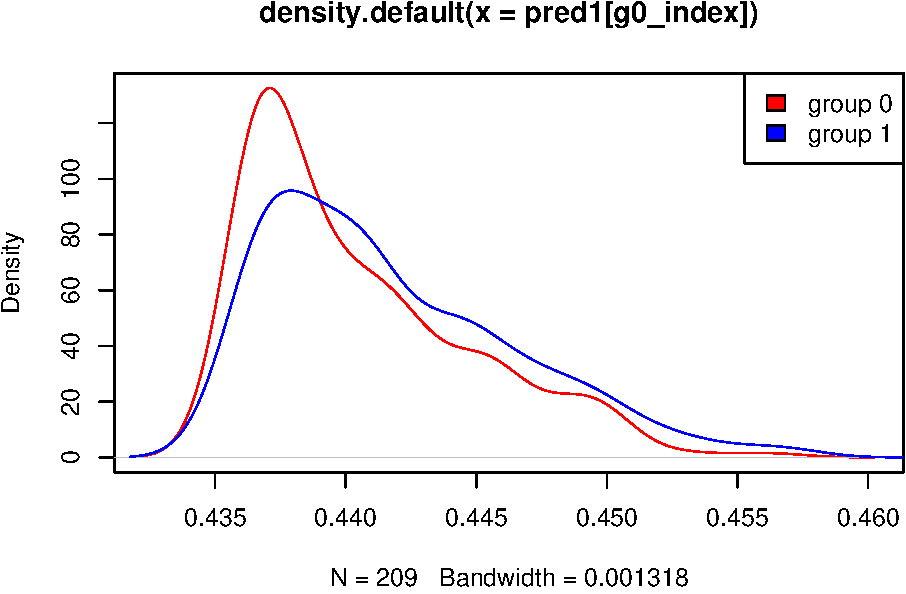
\includegraphics{Main_files/figure-latex/split-1.pdf}

\begin{Shaded}
\begin{Highlighting}[]
\CommentTok{## ATE}

\CommentTok{# build a regression model based on the propensity score}
\CommentTok{# structure the data frame}
\NormalTok{ps1 <-}\StringTok{ }\KeywordTok{predict}\NormalTok{(boost1, high[}\OperatorTok{-}\KeywordTok{c}\NormalTok{(}\DecValTok{1}\NormalTok{,}\DecValTok{2}\NormalTok{)],}\DataTypeTok{n.trees =} \DecValTok{100}\NormalTok{, }\DataTypeTok{type =} \StringTok{'response'}\NormalTok{)}
\NormalTok{df1<-}\KeywordTok{data.frame}\NormalTok{(high}\OperatorTok{$}\NormalTok{Y,high}\OperatorTok{$}\NormalTok{A, ps1)}
\KeywordTok{colnames}\NormalTok{(df1) <-}\StringTok{ }\KeywordTok{c}\NormalTok{(}\StringTok{'Y'}\NormalTok{,}\StringTok{'A'}\NormalTok{,}\StringTok{'PS'}\NormalTok{)}
\NormalTok{model1<-}\KeywordTok{lm}\NormalTok{(df1}\OperatorTok{$}\NormalTok{Y}\OperatorTok{~}\NormalTok{df1}\OperatorTok{$}\NormalTok{A}\OperatorTok{+}\NormalTok{df1}\OperatorTok{$}\NormalTok{PS)}

\NormalTok{end1 <-}\StringTok{ }\KeywordTok{Sys.time}\NormalTok{()}
\end{Highlighting}
\end{Shaded}

\begin{Shaded}
\begin{Highlighting}[]
\CommentTok{#summary(boost1)}
\KeywordTok{summary}\NormalTok{(model1)}
\end{Highlighting}
\end{Shaded}

\begin{verbatim}
## 
## Call:
## lm(formula = df1$Y ~ df1$A + df1$PS)
## 
## Residuals:
##      Min       1Q   Median       3Q      Max 
## -13.4431  -2.6174   0.0114   2.3630  19.8397 
## 
## Coefficients:
##              Estimate Std. Error t value Pr(>|t|)    
## (Intercept) -521.3317     9.6763  -53.88   <2e-16 ***
## df1$A         -3.0830     0.1987  -15.52   <2e-16 ***
## df1$PS      1157.6456    21.9805   52.67   <2e-16 ***
## ---
## Signif. codes:  0 '***' 0.001 '**' 0.01 '*' 0.05 '.' 0.1 ' ' 1
## 
## Residual standard error: 4.296 on 1997 degrees of freedom
## Multiple R-squared:  0.5824, Adjusted R-squared:  0.5819 
## F-statistic:  1392 on 2 and 1997 DF,  p-value: < 2.2e-16
\end{verbatim}

\begin{Shaded}
\begin{Highlighting}[]
\KeywordTok{cat}\NormalTok{(}\StringTok{'The total time using boosted stumps and regression adjustment with high dimension }
\StringTok{    data is:'}\NormalTok{, }
\NormalTok{    end1 }\OperatorTok{-}\StringTok{ }\NormalTok{start1,}\StringTok{'s'}\NormalTok{)}
\end{Highlighting}
\end{Shaded}

\begin{verbatim}
## The total time using boosted stumps and regression adjustment with high dimension 
##     data is: 0.5218561 s
\end{verbatim}

\hypertarget{low-dimension}{%
\subsection{Low Dimension}\label{low-dimension}}

\begin{Shaded}
\begin{Highlighting}[]
\CommentTok{# trani-test split}
\KeywordTok{set.seed}\NormalTok{(}\DecValTok{2021}\NormalTok{)}
\NormalTok{n <-}\StringTok{ }\KeywordTok{nrow}\NormalTok{(low)}
\NormalTok{n_train <-}\StringTok{ }\KeywordTok{round}\NormalTok{(n}\OperatorTok{*}\NormalTok{(}\DecValTok{4}\OperatorTok{/}\DecValTok{5}\NormalTok{),}\DecValTok{0}\NormalTok{)}
\NormalTok{train_idx <-}\StringTok{ }\KeywordTok{sample}\NormalTok{(}\DecValTok{1}\OperatorTok{:}\NormalTok{n,n_train)}
\CommentTok{# test_idx <- setdiff(1:2000, train)}
\NormalTok{train_low <-}\StringTok{ }\NormalTok{low[train_idx,]}
\NormalTok{test_low <-}\StringTok{ }\NormalTok{low[}\OperatorTok{-}\NormalTok{train_idx,]}


\CommentTok{## Propensity Score}
\NormalTok{start0 <-}\StringTok{ }\KeywordTok{Sys.time}\NormalTok{()}

\NormalTok{boost0 =}\StringTok{ }\KeywordTok{gbm}\NormalTok{(A}\OperatorTok{~}\NormalTok{., }\DataTypeTok{data =}\NormalTok{ train_low[}\OperatorTok{-}\DecValTok{1}\NormalTok{], }
            \DataTypeTok{n.trees =} \DecValTok{500}\NormalTok{, }\CommentTok{# the number of trees, 100, 1000. 10000, no big diff}
            \DataTypeTok{shrinkage =} \FloatTok{0.03}\NormalTok{, }\CommentTok{# learning rate, 0.01, 0.03, 0.05, 0.1}
            \DataTypeTok{interaction.depth =} \DecValTok{1} \CommentTok{# depth of each tree, set 1 as stumps}
\NormalTok{            ) }\CommentTok{# here, the parameters we get are from grid search results - }
\end{Highlighting}
\end{Shaded}

\begin{verbatim}
## Distribution not specified, assuming bernoulli ...
\end{verbatim}

\begin{Shaded}
\begin{Highlighting}[]
              \CommentTok{#see the bottom of the file for detail}

\CommentTok{# n.trees <- seq(from = 100, to = 10000, by = 100)}
\CommentTok{# n.trees set the number of trees to be built. Here I choose 1000 manually.}
\NormalTok{pred0 <-}\StringTok{ }\KeywordTok{predict}\NormalTok{(boost0, test_low[}\OperatorTok{-}\KeywordTok{c}\NormalTok{(}\DecValTok{1}\NormalTok{,}\DecValTok{2}\NormalTok{)],}\DataTypeTok{n.trees =} \DecValTok{1000}\NormalTok{, }\DataTypeTok{type =} \StringTok{'response'}\NormalTok{)}
\end{Highlighting}
\end{Shaded}

\begin{verbatim}
## Warning in predict.gbm(boost0, test_low[-c(1, 2)], n.trees = 1000, type =
## "response"): Number of trees not specified or exceeded number fit so far. Using
## 500.
\end{verbatim}

\begin{Shaded}
\begin{Highlighting}[]
\CommentTok{# plot by A to see the distribution of the predicted value}
\NormalTok{g0_index <-}\StringTok{ }\NormalTok{test_low}\OperatorTok{$}\NormalTok{A }\OperatorTok{==}\StringTok{ }\DecValTok{0}
\NormalTok{g1_index <-}\StringTok{ }\NormalTok{test_low}\OperatorTok{$}\NormalTok{A }\OperatorTok{==}\StringTok{ }\DecValTok{1}
\KeywordTok{plot}\NormalTok{(}\KeywordTok{density}\NormalTok{(pred0[g0_index]),}\DataTypeTok{col =} \StringTok{'red'}\NormalTok{)}
\KeywordTok{lines}\NormalTok{(}\KeywordTok{density}\NormalTok{(pred0[g1_index]),}\DataTypeTok{col =} \StringTok{'blue'}\NormalTok{)}
\KeywordTok{legend}\NormalTok{(}\StringTok{'topright'}\NormalTok{,}\DataTypeTok{legend =} \KeywordTok{c}\NormalTok{(}\StringTok{'group 0'}\NormalTok{,}\StringTok{'group 1'}\NormalTok{),}\DataTypeTok{fill =} \KeywordTok{c}\NormalTok{(}\StringTok{'red'}\NormalTok{,}\StringTok{'blue'}\NormalTok{))}
\end{Highlighting}
\end{Shaded}

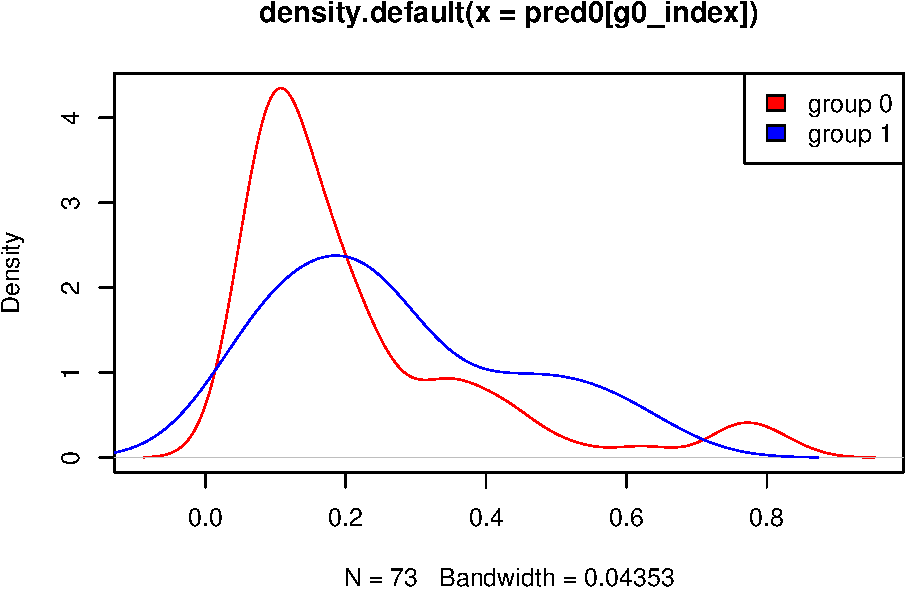
\includegraphics{Main_files/figure-latex/unnamed-chunk-12-1.pdf}

\begin{Shaded}
\begin{Highlighting}[]
\CommentTok{## ATE}

\CommentTok{# build a regression model based on the propensity score}
\CommentTok{# structure the data frame}
\NormalTok{ps0 <-}\StringTok{ }\KeywordTok{predict}\NormalTok{(boost0, low[}\OperatorTok{-}\KeywordTok{c}\NormalTok{(}\DecValTok{1}\NormalTok{,}\DecValTok{2}\NormalTok{)],}\DataTypeTok{n.trees =} \DecValTok{100}\NormalTok{, }\DataTypeTok{type =} \StringTok{'response'}\NormalTok{)}
\NormalTok{df0<-}\KeywordTok{data.frame}\NormalTok{(low}\OperatorTok{$}\NormalTok{Y,low}\OperatorTok{$}\NormalTok{A, ps0)}
\KeywordTok{colnames}\NormalTok{(df0) <-}\StringTok{ }\KeywordTok{c}\NormalTok{(}\StringTok{'Y'}\NormalTok{,}\StringTok{'A'}\NormalTok{,}\StringTok{'PS'}\NormalTok{)}
\NormalTok{model0<-}\KeywordTok{lm}\NormalTok{(df0}\OperatorTok{$}\NormalTok{Y}\OperatorTok{~}\NormalTok{df0}\OperatorTok{$}\NormalTok{A}\OperatorTok{+}\NormalTok{df0}\OperatorTok{$}\NormalTok{PS)}

\NormalTok{end0 <-}\StringTok{ }\KeywordTok{Sys.time}\NormalTok{()}
\end{Highlighting}
\end{Shaded}

\begin{Shaded}
\begin{Highlighting}[]
\CommentTok{# summary(boost0)}
\KeywordTok{summary}\NormalTok{(model0)}
\end{Highlighting}
\end{Shaded}

\begin{verbatim}
## 
## Call:
## lm(formula = df0$Y ~ df0$A + df0$PS)
## 
## Residuals:
##      Min       1Q   Median       3Q      Max 
## -10.9058  -2.2172  -0.5321   1.0805  27.7107 
## 
## Coefficients:
##             Estimate Std. Error t value Pr(>|t|)    
## (Intercept)  11.5946     0.3589  32.310  < 2e-16 ***
## df0$A         2.5271     0.4101   6.162 1.54e-09 ***
## df0$PS       22.3931     1.4479  15.466  < 2e-16 ***
## ---
## Signif. codes:  0 '***' 0.001 '**' 0.01 '*' 0.05 '.' 0.1 ' ' 1
## 
## Residual standard error: 3.495 on 472 degrees of freedom
## Multiple R-squared:  0.4672, Adjusted R-squared:  0.465 
## F-statistic:   207 on 2 and 472 DF,  p-value: < 2.2e-16
\end{verbatim}

\begin{Shaded}
\begin{Highlighting}[]
\KeywordTok{cat}\NormalTok{(}\StringTok{'The total time using boosted stumps and regression adjustment with low dimension }
\StringTok{    data is:'}\NormalTok{, end0 }\OperatorTok{-}\StringTok{ }\NormalTok{start0,}\StringTok{'s'}\NormalTok{)}
\end{Highlighting}
\end{Shaded}

\begin{verbatim}
## The total time using boosted stumps and regression adjustment with low dimension 
##     data is: 0.08484101 s
\end{verbatim}

\hypertarget{additional-code-grid-search}{%
\subsection{Additional Code: Grid
Search}\label{additional-code-grid-search}}

In this part, we included our code for conducting grid search for
lowdim. The procedure is similar in highdim. For the readability of the
file, we choose to comment out the code.

\begin{Shaded}
\begin{Highlighting}[]
\CommentTok{# grid search}
\CommentTok{# hyper_grid_low1 <- expand.grid(}
\CommentTok{#  shrinkage = c(.01, 0.03, 0.05),}
\CommentTok{#  interaction.depth = 1 - since it is boosted stumps}
\CommentTok{#  n.minobsinnode = c(5, 10, 15),}
\CommentTok{#  bag.fraction = c(.65, .8, 1), }
\CommentTok{#  optimal_trees = 0,               # a place to dump results}
\CommentTok{#  min_RMSE = 0                     # a place to dump results}
\CommentTok{#)}

\CommentTok{# randomize data}
\CommentTok{# random_index <- sample(1:nrow(train_low), nrow(train_low))}
\CommentTok{# random_ames_train <- train_low[random_index, ]}

\CommentTok{# grid search }
\CommentTok{# for(i in 1:nrow(hyper_grid_low1)) \{}
  \CommentTok{# reproducibility}
\CommentTok{#  set.seed(2020)}
  \CommentTok{# train model}
\CommentTok{#  gbm.tune <- gbm(}
\CommentTok{#    formula = A~.,}
\CommentTok{#    data = train_low[-1],}
\CommentTok{#    n.trees = 500,}
\CommentTok{#    interaction.depth = hyper_grid_low1$interaction.depth[i],}
\CommentTok{#    shrinkage = hyper_grid_low1$shrinkage[i],}
\CommentTok{#    n.minobsinnode = hyper_grid_low1$n.minobsinnode[i],}
\CommentTok{#  bag.fraction = hyper_grid_low1$bag.fraction[i],}
\CommentTok{#   train.fraction = .75,}
\CommentTok{#    n.cores = NULL, # will use all cores by default}
\CommentTok{#    verbose = FALSE}
\CommentTok{#  )}

  \CommentTok{# add min training error and trees to grid}
\CommentTok{#  hyper_grid_low1$optimal_trees[i] <- which.min(gbm.tune$valid.error)}
\CommentTok{#  hyper_grid_low1$min_RMSE[i] <- sqrt(min(gbm.tune$valid.error))}
\CommentTok{# \}}

\CommentTok{# hyper_grid_low1 %>% }
\CommentTok{# dplyr::arrange(min_RMSE) %>%}
\CommentTok{#  head(10)}
\end{Highlighting}
\end{Shaded}

\hypertarget{conclusion}{%
\subsection{Conclusion}\label{conclusion}}

\begin{Shaded}
\begin{Highlighting}[]
\KeywordTok{data.frame}\NormalTok{(}\DataTypeTok{ATE=}\KeywordTok{c}\NormalTok{(}\KeywordTok{round}\NormalTok{(model1}\OperatorTok{$}\NormalTok{coefficients[}\DecValTok{2}\NormalTok{],}\DecValTok{4}\NormalTok{),}
                 \KeywordTok{round}\NormalTok{(model0}\OperatorTok{$}\NormalTok{coefficients[}\DecValTok{2}\NormalTok{],}\DecValTok{3}\NormalTok{)), }\DataTypeTok{True.ATE=}\KeywordTok{c}\NormalTok{(true_ATE_high,true_ATE_low), }
                  \DataTypeTok{diff=}\KeywordTok{c}\NormalTok{(}\KeywordTok{round}\NormalTok{(true_ATE_high }\OperatorTok{-}\StringTok{ }\NormalTok{model1}\OperatorTok{$}\NormalTok{coefficients[}\DecValTok{2}\NormalTok{],}\DecValTok{3}\NormalTok{),}
                         \KeywordTok{round}\NormalTok{(true_ATE_low }\OperatorTok{-}\StringTok{ }\NormalTok{model0}\OperatorTok{$}\NormalTok{coefficients[}\DecValTok{2}\NormalTok{],}\DecValTok{3}\NormalTok{)),}
                  \DataTypeTok{time=}\KeywordTok{c}\NormalTok{(end1}\OperatorTok{-}\NormalTok{start1,end0}\OperatorTok{-}\NormalTok{start0),}\DataTypeTok{row.names =} \KeywordTok{c}\NormalTok{(}\StringTok{'HighDim'}\NormalTok{, }\StringTok{'LowDim'}\NormalTok{))}
\end{Highlighting}
\end{Shaded}

\begin{verbatim}
##            ATE True.ATE   diff            time
## HighDim -3.083     -3.0  0.083 0.52185607 secs
## LowDim   2.527      2.5 -0.027 0.08484101 secs
\end{verbatim}

The density plots show the matching of propensity scores between the two
groups. The boosted stumps performs well on both of the datasets as they
show the density plots between two groups overlap each other on a large
scale. For the parameters of the regression model, higher dimension data
requires smaller learning rate and less number of trees. I would suggest
to use the combination on higher dimension datasets, as the boosting
stumps identifying variable relative influence effectively and produces
well-matched propensity scores between the experiment group and the
control group.

\hypertarget{algo-3-15-a4-regression-estimate}{%
\section{Algo 3: 15 A4 Regression
Estimate}\label{algo-3-15-a4-regression-estimate}}

\hypertarget{methodology}{%
\subsection{Methodology}\label{methodology}}

Regression Estimate is a really simple estimation model to the calculate
ATE, which do not require Propensity Scores calculation. This makes it a
straight forward model and a computational efficient model. By
implementing the linear regression on treated groups and untreated
groups, we could regress on different groups to get the two different
sets of paramaters and then by predicting the models on the whole
dataset, substracting the prediction we can get the difference between
the two regression models. In the end, we can calculate the ATE(Average
Treatment Effect) by taking the average of the difference.

\[ ATE = N^{-1} \sum^N_{i=1}(\hat {m_1}(X_i)-\hat {m_0}(X_i))\]

Denote that

\(N\) is the number of samples in the dataset,

\(X_i\) is the datapoint in the dataset,

\(m_1\) is the regression model learned from the treated groups,

\(m_0\) is the regression model learned from the untreated groups,

\(\hat {m_1}(X_i)\) is the prediction of the regression model \(m_1\) on
the datapoint \(X_i\),

\(\hat {m_0}(X_i)\) is the prediction of the regression model \(m_0\) on
the datapoint \(X_i\).

\hypertarget{implementation}{%
\subsection{Implementation}\label{implementation}}

\begin{Shaded}
\begin{Highlighting}[]
\CommentTok{# Read the data and split the data into two groups -- Treated Group and Untreated Group}

\NormalTok{high_data <-}\KeywordTok{read.csv}\NormalTok{(}\StringTok{'../data/highDim_dataset.csv'}\NormalTok{)}
\NormalTok{low_data <-}\KeywordTok{read.csv}\NormalTok{(}\StringTok{'../data/lowDim_dataset.csv'}\NormalTok{)}

\NormalTok{N_high <-}\StringTok{ }\KeywordTok{dim}\NormalTok{(high_data)[}\DecValTok{1}\NormalTok{]}
\NormalTok{N_low <-}\StringTok{ }\KeywordTok{dim}\NormalTok{(low_data)[}\DecValTok{1}\NormalTok{]}

\NormalTok{high_data_X <-}\StringTok{ }\NormalTok{high_data[,}\DecValTok{3}\OperatorTok{:}\KeywordTok{dim}\NormalTok{(high_data)[}\DecValTok{2}\NormalTok{]]}
\NormalTok{low_data_X <-}\StringTok{ }\NormalTok{low_data[,}\DecValTok{3}\OperatorTok{:}\KeywordTok{dim}\NormalTok{(low_data)[}\DecValTok{2}\NormalTok{]]}

\NormalTok{high_treated <-}\StringTok{ }\NormalTok{high_data[high_data}\OperatorTok{$}\NormalTok{A}\OperatorTok{==}\DecValTok{1}\NormalTok{,}\OperatorTok{-}\DecValTok{2}\NormalTok{]}
\NormalTok{high_untreated <-}\StringTok{ }\NormalTok{high_data[high_data}\OperatorTok{$}\NormalTok{A}\OperatorTok{==}\DecValTok{0}\NormalTok{,}\OperatorTok{-}\DecValTok{2}\NormalTok{]}

\NormalTok{N_high_treated <-}\StringTok{ }\KeywordTok{dim}\NormalTok{(high_treated)[}\DecValTok{1}\NormalTok{]}
\NormalTok{N_high_untreated <-}\StringTok{ }\KeywordTok{dim}\NormalTok{(high_untreated)[}\DecValTok{1}\NormalTok{]}

\NormalTok{low_treated <-}\StringTok{ }\NormalTok{low_data[low_data}\OperatorTok{$}\NormalTok{A}\OperatorTok{==}\DecValTok{1}\NormalTok{,}\OperatorTok{-}\DecValTok{2}\NormalTok{]}
\NormalTok{low_untreated <-}\StringTok{ }\NormalTok{low_data[low_data}\OperatorTok{$}\NormalTok{A}\OperatorTok{==}\DecValTok{0}\NormalTok{,}\OperatorTok{-}\DecValTok{2}\NormalTok{]}

\NormalTok{N_low_treated <-}\StringTok{ }\KeywordTok{dim}\NormalTok{(low_treated)[}\DecValTok{1}\NormalTok{]}
\NormalTok{N_low_untreated <-}\StringTok{ }\KeywordTok{dim}\NormalTok{(low_untreated)[}\DecValTok{1}\NormalTok{]}

\CommentTok{# Train the data and record the training time of two datasets}

\NormalTok{time<-}\StringTok{ }\KeywordTok{system.time}\NormalTok{(\{}
\NormalTok{  high_treated_lm <-}\StringTok{ }\KeywordTok{lm}\NormalTok{(Y}\OperatorTok{~}\NormalTok{.,}\DataTypeTok{data =}\NormalTok{ high_treated);}
\NormalTok{  high_untreated_lm <-}\StringTok{ }\KeywordTok{lm}\NormalTok{(Y}\OperatorTok{~}\NormalTok{.,}\DataTypeTok{data =}\NormalTok{ high_untreated);}
\NormalTok{  high_treated_predict_all <-}\StringTok{ }\KeywordTok{predict}\NormalTok{(high_treated_lm,}\DataTypeTok{newdata =}\NormalTok{ high_data_X);}
\NormalTok{  high_untreated_predict_all <-}\StringTok{ }\KeywordTok{predict}\NormalTok{(high_untreated_lm,}\DataTypeTok{newdata =}\NormalTok{ high_data_X)\})}
\NormalTok{train_time_high <-}\StringTok{ }\NormalTok{time[}\DecValTok{1}\NormalTok{]}
\CommentTok{#train_time_high}

\NormalTok{time<-}\StringTok{ }\KeywordTok{system.time}\NormalTok{(\{}
\NormalTok{  low_treated_lm <-}\StringTok{ }\KeywordTok{lm}\NormalTok{(Y}\OperatorTok{~}\NormalTok{.,}\DataTypeTok{data =}\NormalTok{ low_treated);}
\NormalTok{  low_untreated_lm <-}\StringTok{ }\KeywordTok{lm}\NormalTok{(Y}\OperatorTok{~}\NormalTok{.,}\DataTypeTok{data =}\NormalTok{ low_untreated);}
\NormalTok{  low_treated_predict_all <-}\StringTok{ }\KeywordTok{predict}\NormalTok{(low_treated_lm,}\DataTypeTok{newdata =}\NormalTok{ low_data_X);}
\NormalTok{  low_untreated_predict_all <-}\StringTok{ }\KeywordTok{predict}\NormalTok{(low_untreated_lm,}\DataTypeTok{newdata =}\NormalTok{ low_data_X)\})}
\NormalTok{train_time_low <-}\StringTok{ }\NormalTok{time[}\DecValTok{1}\NormalTok{]}
\CommentTok{#train_time_low}

\CommentTok{# Calculate the ATE}

\NormalTok{reg_est_ATE_high<-}\KeywordTok{sum}\NormalTok{(high_treated_predict_all }\OperatorTok{-}\StringTok{ }\NormalTok{high_untreated_predict_all)}\OperatorTok{/}\NormalTok{N_high}
\NormalTok{reg_est_ATE_low<-}\KeywordTok{sum}\NormalTok{(low_treated_predict_all }\OperatorTok{-}\StringTok{ }\NormalTok{low_untreated_predict_all)}\OperatorTok{/}\NormalTok{N_low}
\CommentTok{#reg_est_ATE_high}
\CommentTok{#reg_est_ATE_low}
\end{Highlighting}
\end{Shaded}

\hypertarget{conclustions}{%
\subsection{Conclustions}\label{conclustions}}

\begin{Shaded}
\begin{Highlighting}[]
\KeywordTok{data.frame}\NormalTok{(}\DataTypeTok{ATE=}\KeywordTok{c}\NormalTok{(}\KeywordTok{round}\NormalTok{(reg_est_ATE_high,}\DecValTok{4}\NormalTok{),}
                 \KeywordTok{round}\NormalTok{(reg_est_ATE_low,}\DecValTok{4}\NormalTok{)), }\DataTypeTok{True.ATE=}\KeywordTok{c}\NormalTok{(true_ATE_high,true_ATE_low), }
                  \DataTypeTok{diff=}\KeywordTok{c}\NormalTok{(}\KeywordTok{round}\NormalTok{(true_ATE_high }\OperatorTok{-}\StringTok{ }\NormalTok{model1}\OperatorTok{$}\NormalTok{coefficients[}\DecValTok{2}\NormalTok{],}\DecValTok{3}\NormalTok{),}
                         \KeywordTok{round}\NormalTok{(true_ATE_low }\OperatorTok{-}\StringTok{ }\NormalTok{model0}\OperatorTok{$}\NormalTok{coefficients[}\DecValTok{2}\NormalTok{],}\DecValTok{3}\NormalTok{)),}
                  \DataTypeTok{time=}\KeywordTok{c}\NormalTok{(train_time_high,train_time_low),}\DataTypeTok{row.names =} \KeywordTok{c}\NormalTok{(}\StringTok{'HighDim'}\NormalTok{, }\StringTok{'LowDim'}\NormalTok{))}
\end{Highlighting}
\end{Shaded}

\begin{verbatim}
##             ATE True.ATE   diff  time
## HighDim -2.9598     -3.0  0.083 0.104
## LowDim   2.5269      2.5 -0.027 0.008
\end{verbatim}

We can conclude that the model is more fit to the low dimension dataset.
With higher dimension, the ATE has higher bias rate(1.34\% vs 1.08\%).

\hypertarget{summary}{%
\section{Summary}\label{summary}}

\textbf{Comparision among the three models}

The table shows the result of the three algorithm's ATE in the two
different datasets.

\begin{longtable}[]{@{}lllll@{}}
\toprule
Algorithm & \textbf{ATE High} & difference & \textbf{ATE Low} &
difference\tabularnewline
\midrule
\endhead
True ATE & -3 & - & 2.5 & -\tabularnewline
Doubly Robust Estimation + Boosted Stumps & -2.9626 & 2.5187 & 0.0374 &
0.0187\tabularnewline
Regression Adjustment + Boosted Stumps & -3.0830 & 2.5271 & 0.0830 &
0.0271\tabularnewline
Regression Estimate & -2.9598 & 2.5269 & 0.0402 & 0.0269\tabularnewline
\bottomrule
\end{longtable}

All of the models are well-performed after tuning. From the table above,
we can see that the Doubly Robust Estimation + Boosted Stumps model has
the smallest difference with the true ATE on both of the datasets.
Results of Regression Estimate and Regression adjustment are close on
the high dimension datasets while the former model outperformed on low
dimension.

\begin{longtable}[]{@{}lll@{}}
\toprule
Algorithm & Training Time High & Training Time Low\tabularnewline
\midrule
\endhead
Doubly Robust Estimation + Boosted Stumps & 1.2180 &
0.0230\tabularnewline
Regression Estimate & 0.2270 & 0.0190\tabularnewline
Regression Adjustment + Boosted Stumps & 0.5060 & 0.1287\tabularnewline
\bottomrule
\end{longtable}

Comparing the training time on each of the methods and the datasets, the
regression estimate has the shortest training time on both of the
datasets. Regression adjustment + boosted stumps have a shorter training
time than doubly robust estimation on the high dimension dataset, but
six times longer on the low dimension dataset. We conclude that the
regression estimate is more computationally efficient than the Doubly
Robust Estimation + Boosted Stumps model.

For model flexibility, we would recommend Doubly Robust Estimation +
Boosted Stumps, as it can be customized with grid search and achieve
higher accuracy for high and low dimension data. For efficiency, the
Regression Estimate would give an informative idea of the ATE between
the experiment and the control group in a productive manner.

\end{document}
